%! Author = danielmendes
%! Date = 29.11.24

\chapter{Optimierungen von Datentypen}

\section{Allgemeine Faktoren}

Bei der Auswahl von Datentypen gibt es viele Faktoren, die Einfluss auf die Performance haben können.
Einige von diesen Faktoren sind abhängig vom jeweils gewählten Datentyp, andere sind dafür genereller anwendbar.
Zu den allgemeinen Einflussfaktoren kommen wir zunächst und anschließend betrachten wir die einzelnen Typen wie Ganzzahlen oder Strings im Detail an.

Allgemein gilt bei Datentypen, dass kleiner besser ist, weshalb man den kleinstmöglichen Datentypen wählen sollte, den man speichern kann und der die vorhandenen Daten entsprechend repräsentieren kann.
Dadurch wird weniger Speicherplatz (In-Memory und CPU-Cache) in Anspruch genommen, weshalb die Abfragen meistens schneller sind.
Ein weiterer Vorteil, der für die Benutzung von kleinstmöglichen Typen spricht, ist die einfache Typveränderung, wenn man die vorhandenen Daten falsch eingeschätzt hat und nachträglich ein größerer Datentyp benötigt wird.

%TODO (Daniel): add grafix and analysis
Ein weiterer allgemeiner Leitsatz ist, dass ein einfacherer Datentyp gut ist, denn es werden weniger CPU-Zyklen benötigt, um Operationen auf einfacheren Datentypen zu verarbeiten.
Beispielweise ist Integer einfacher zu verarbeiten als Character, da Character Sets und Sortierregeln den Character-Vergleich erschweren.
%TODO (Daniel): add grafix and analysis

Generell bringt es auch Performancegewinne, wenn man NULL vermeidet, wenn es möglich ist.
Viele Tabellen enthalten NULLABLE Spalten, selbst wenn die Anwendung kein NULL (Fehlen eines Wertes) speichern muss, da dies die Standardeinstellung ist.
Daher ist am besten solche Spalten bei der Tabellenerstellung mit dem Identifier NOT NULL zu definieren.
Wenn allerdings NULL-Werte gespeichert werden soll, dann sollte der Identifier nicht genutzt werden und für MySQL ist es dann schwieriger Abfragen zu optimieren, da durch Indizes, Indexstatistiken und Wertevergleiche komplizierter werden.
Dadurch benötigen sie auch mehr Speicherplatz und erfordern eine spezielle Verarbeitung innerhalb von MySQL.
Das liegt daran, dass indizierte nullable Spalten ein zusätzliches Byte pro Eintrag gebrauchen und das kann dazu führen, dass ein Index mit fester Größe in einen variablen Index umgewandelt wird.
Die Leistungsverbesserung, die durch die Änderung von NULL-Spalten in NOT NULL erzielt wird, ist in der Regel gering, aber bei der Verwendung von Indizes sollte besonders darauf geachtet werden.
%TODO (Daniel): add grafix and analysis

Wenn man bei der Erstellung von Tabellen nicht sicher ist, welchen Datentypen für die Spalten geeignet sind, bieten sich folgende Schritte für die Auswahl von Datentypen an.
Als Erstes sollte die allgemeine Klasse von Typen, z.B. numerisch, Zeichenketten oder zeitbezogen, bestimmt werden.
Daraufhin sollte der spezifische Typ gewählt werden.
Viele können dieselbe Art von Daten speichern, unterscheiden sich jedoch im Bereich der Werte, die sie speichern können.
Auch sind sie unterschiedlich in der Genauigkeit (precision), die sie erlauben und dem physischen Speicherplatz, den sie entweder auf der Festplatte oder im Arbeitsspeicher benötigen.
Einige Datentypen haben auch spezielle Verhaltensweisen und Eigenschaften.

\section{Einzelne Datentypen und weitere Faktoren}
DATETIME und TIMESTAMP können dieselbe Art von Daten speichern und beide haben dabei eine Genauigkeit von einer Sekunde.
TIMESTAMP benötigt aber nur halb so viel Speicherplatz, ist zeitzonenbewusst und verfügt über spezielle Auto-Update-Funktionen.
Allerdings hat TIMESTAMP einen viel kleineren Bereich an erlaubten Werten und manchmal können seine speziellen Fähigkeiten ein Nachteil sein.
(TODO (Daniel): add rest oft ext here).

MySQL unterstützt auch viele Aliase, z.B. INTEGER, BOOL, NUMERIC.
Diese Aliase können verwirrend sein, sie beeinflussen aber nicht die Performance.
Erkennen kann das an, wenn man eine Tabelle mit einem aliasierten Datentyp erstellt und dann mit SHOW CREATE TABLE die Tabelle untersucht.
Denn tatsächlich würde man anstelle des aliasierten Datentypen den Basistyp angezeigt bekommen, da intern der aliasierte Datentyp gegen diesen umgewandelt wird.


\begin{figure}[!ht]
    \centering
    \begin{subfigure}[t]{0.48\textwidth}
        \centering
        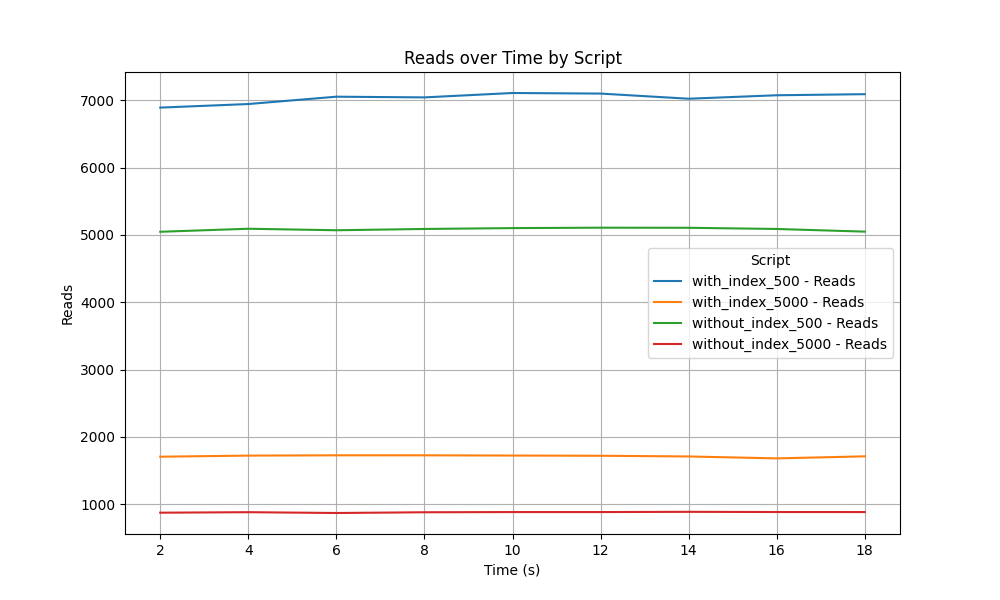
\includegraphics[width=\textwidth]{PNGs/Index/B-Tree/High_Reads}
        \label{high-reads}
    \end{subfigure}
    \hfill
    \begin{subfigure}[t]{0.48\textwidth}
        \centering
        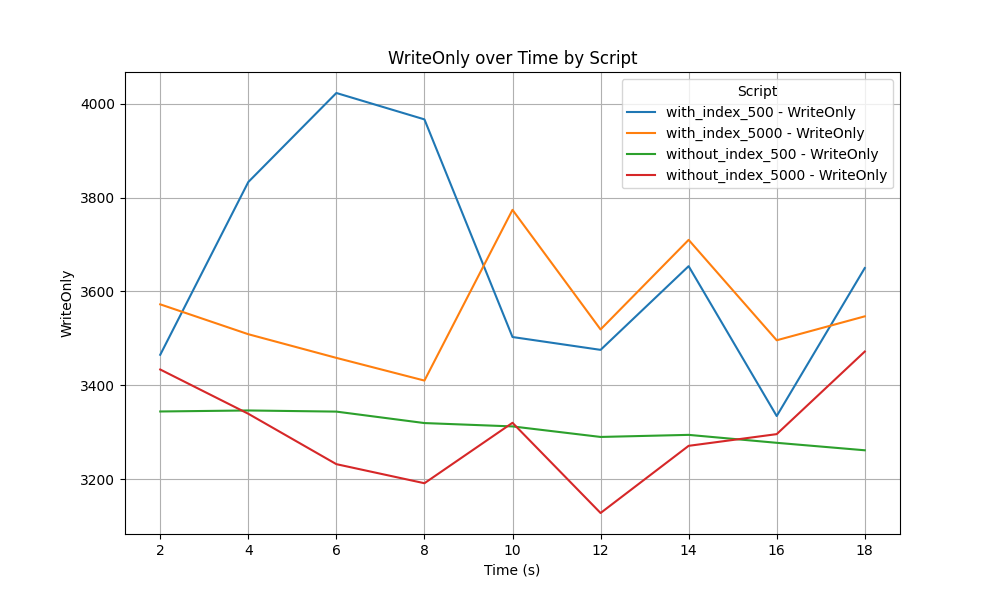
\includegraphics[width=\textwidth]{PNGs/Index/B-Tree/High_Writes}
        \label{high-writes}
    \end{subfigure}
    \caption[High-Counts: Reads und Writes]{Grafik zeigt die verschiedenen Zeiten (in ms) für Readsabfragen (links) und Schreibbefehle (rechts) mit 500 bzw. 5000 Zeilen}
    \label{fig:high-b-tree-columns}
\end{figure}

\begin{figure}[!ht]
    \centering
    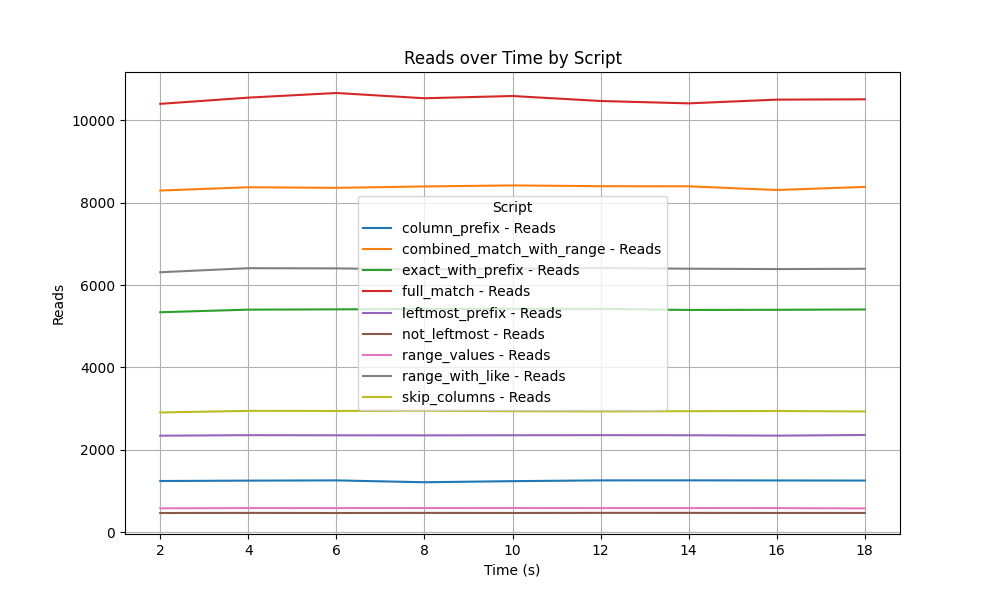
\includegraphics[width=.8\textwidth]{PNGs/Index/B-Tree/Query_Reads}
    \caption[B - Tree - Selects - Ergebnis]{Grafik visualisiert die Unterschiede von verschieden Select - Queries auf dieselben Daten. Je nach Gewschiwndikeit greift der Index besser oder nicht }
    \label{fig:b-tree-query-reads}
\end{figure}